\documentclass[a4paper,12pt]{article}
\usepackage{graphicx}
\usepackage{amsmath}
\usepackage{geometry}
\geometry{margin=1in}
\usepackage{polyglossia}
\setmainlanguage{english}
\setotherlanguage[numerals=hindu]{urdu}

% Use Noto Nastaliq Urdu or Jameel Noori Nastaleeq for better Urdu support
\newfontfamily\urdufont[
Script=Arabic,
Language=Urdu,
Scale=0.8,
AutoFakeBold=1.0,
AutoFakeSlant=0.15
]{Noto Nastaliq Urdu}

% Adjust paragraph settings
\setlength{\parindent}{0pt}
\setlength{\parskip}{0.5em}

% Define Urdu text command with proper alignment
\newcommand{\urdutextblock}[1]{%
	\begin{urdu}%
			\large\urdufont #1%
	\end{urdu}%
}

\newcommand{\urdusection}[1]{%
	\section*{\begin{center}\begin{urdu}\large\urdufont #1\end{urdu}\end{center}}%
}
	
	\begin{document}
		
		% English Report
		\title{SIP and SWP Report}
		\author{}
		\date{\today}
		\maketitle
		
		\section{Abstract}
		This report explains a savings and withdrawal plan over 60 years. It includes 20 years of saving money (SIP) and 40 years of withdrawing money (SWP). Simple charts and explanations are given.
		
		\section{Introduction}
		Systematic Investment Plans (SIPs) and Systematic Withdrawal Plans (SWPs) are financial tools designed to help individuals achieve long-term savings and income goals. An SIP allows an individual to invest a fixed amount of money regularly into a mutual fund or other investment vehicles. This disciplined approach encourages consistent savings and takes advantage of market fluctuations through rupee-cost averaging. In contrast, SWP enables an individual to withdraw a fixed or variable amount of money from their investments periodically, providing a steady income stream while keeping the remaining investments potentially growing. 
		
		Both SIPs and SWPs are beneficial for creating a financial corpus during the earning phase and systematically utilizing it during the retirement or other income-needing phases. This report demonstrates how combining SIPs and SWPs creates a sustainable financial plan over decades.
		
		\section{SIP Phase Analysis}
		During the first 20 years, savings grow because money is added regularly and earns interest. Figure~\ref{fig:sip-phase} shows how savings grow over time.
		

\begin{figure}[!h]
	\centering
	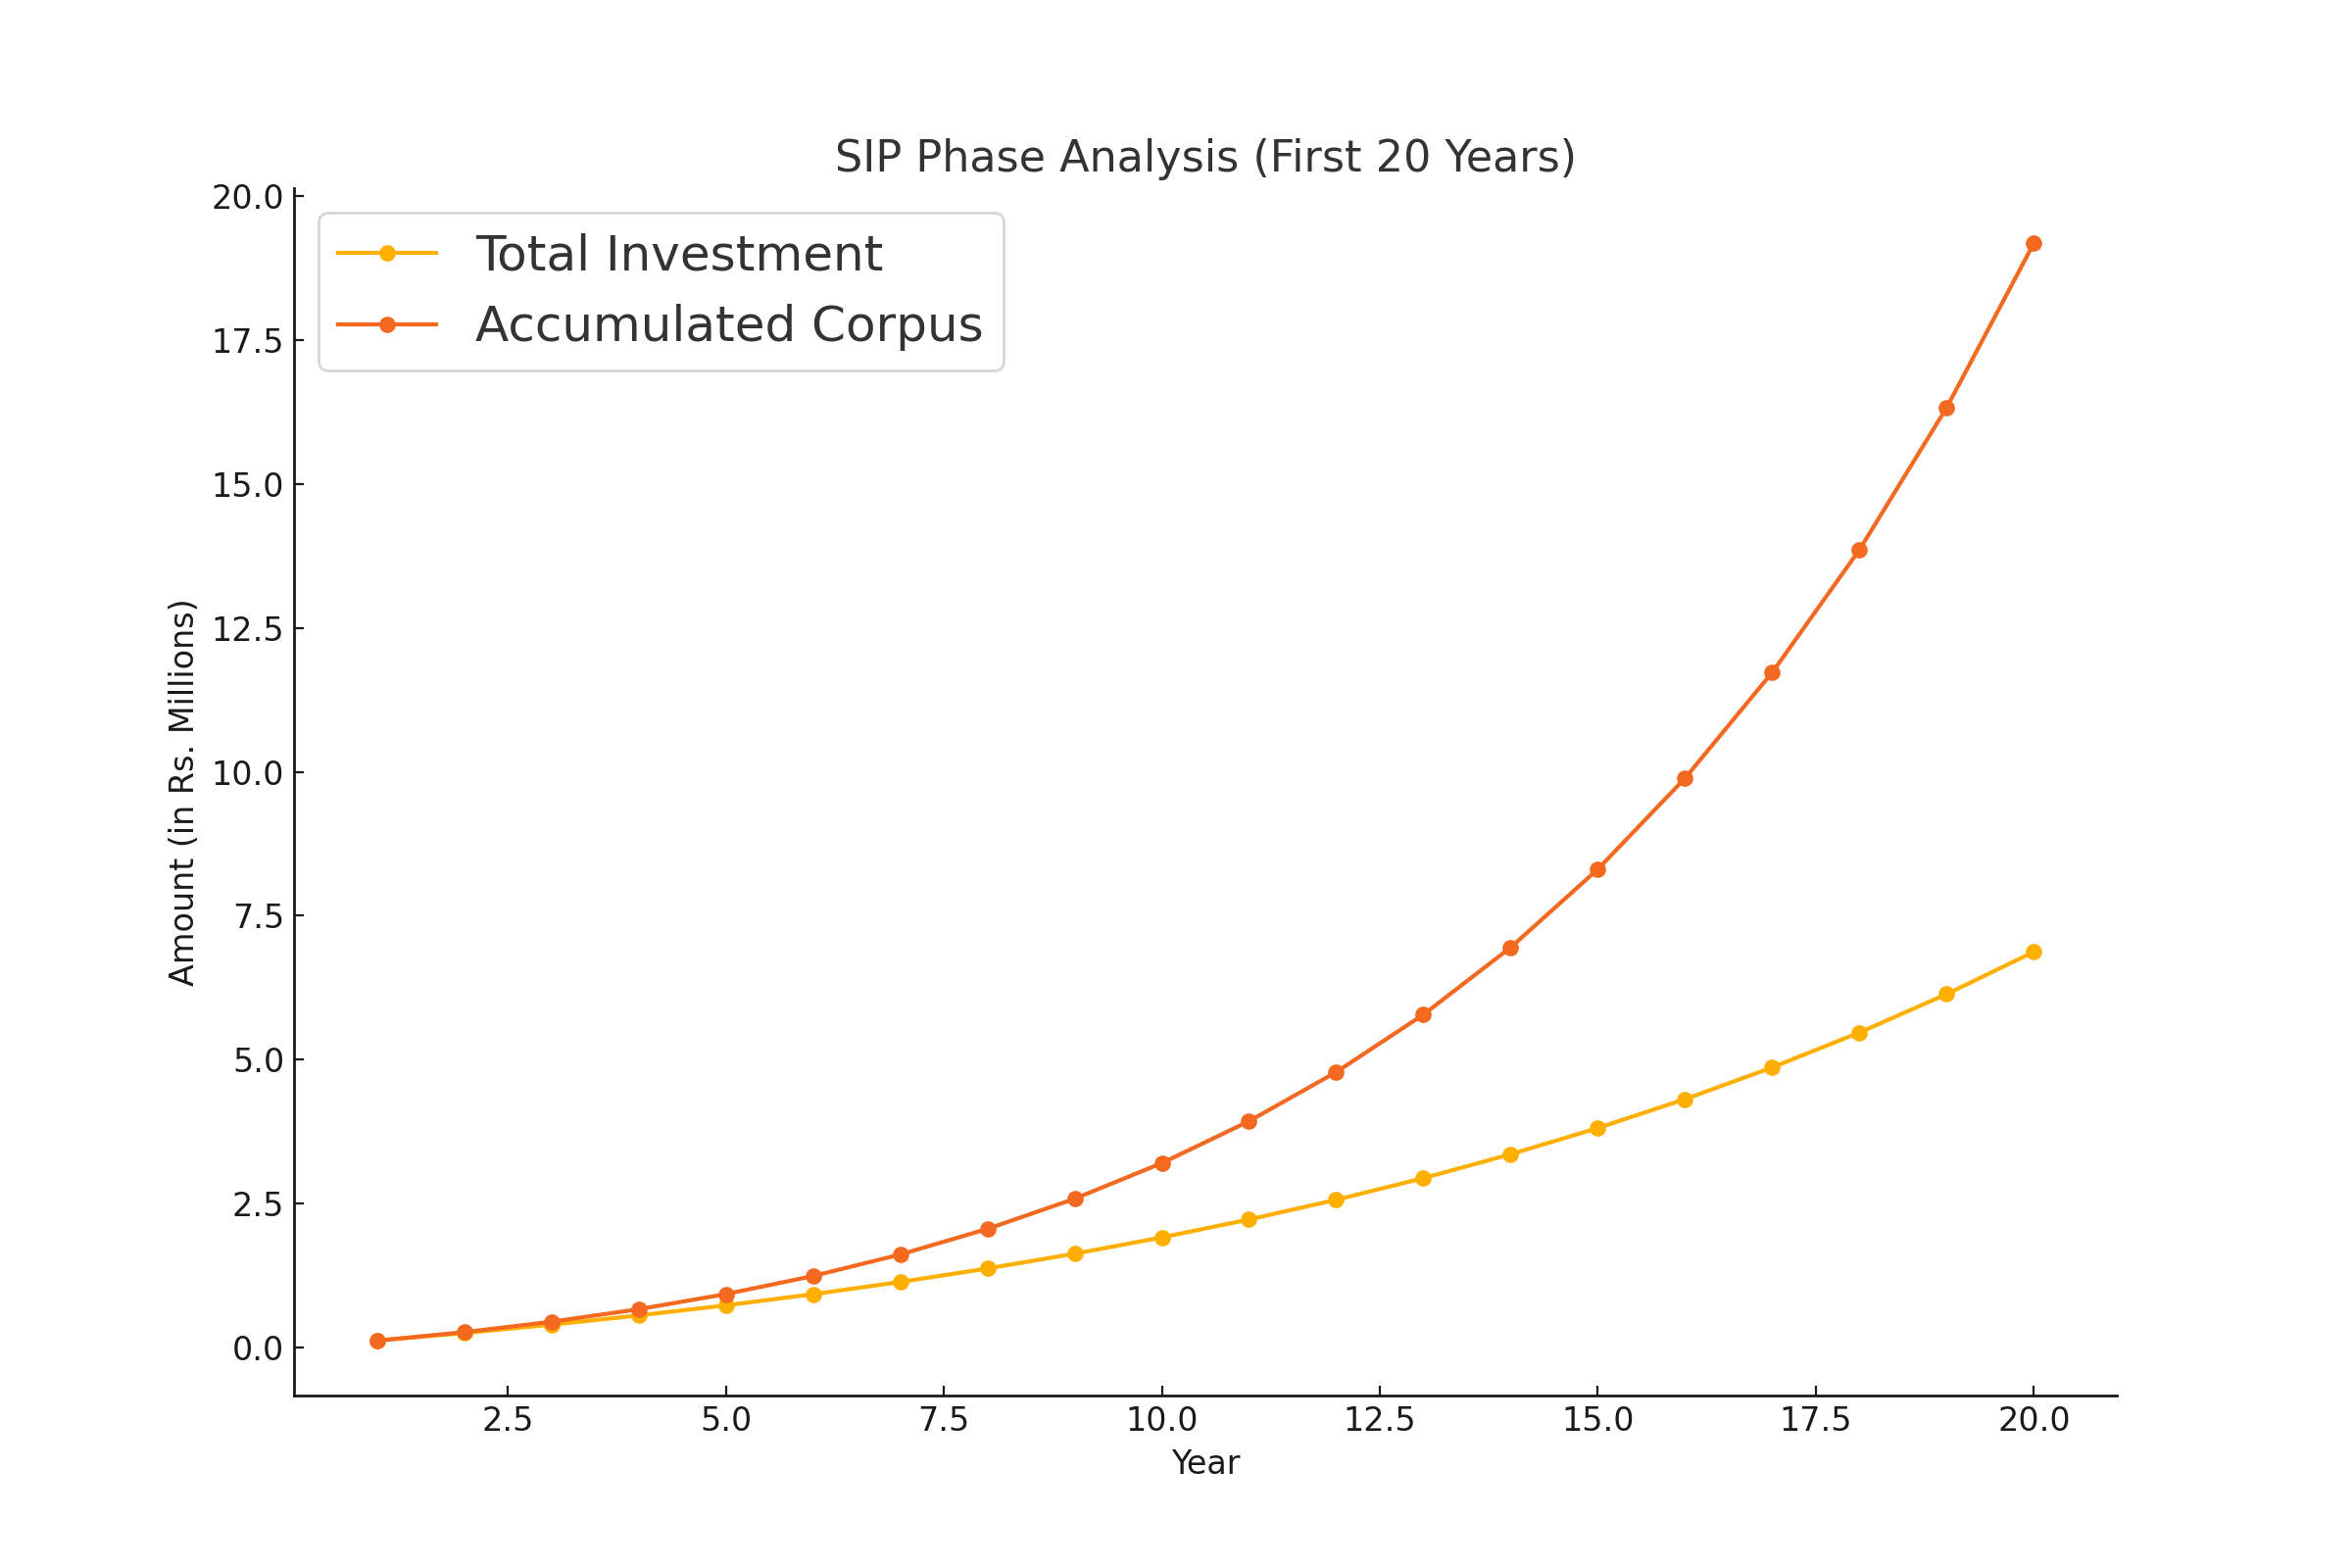
\includegraphics[width=0.6\textwidth]{sip_phase_plot.png}
	\caption{SIP Phase (Years 1 to 20)}
	\label{fig:sip-phase}
\end{figure}

\begin{figure}[!h]
	\centering
	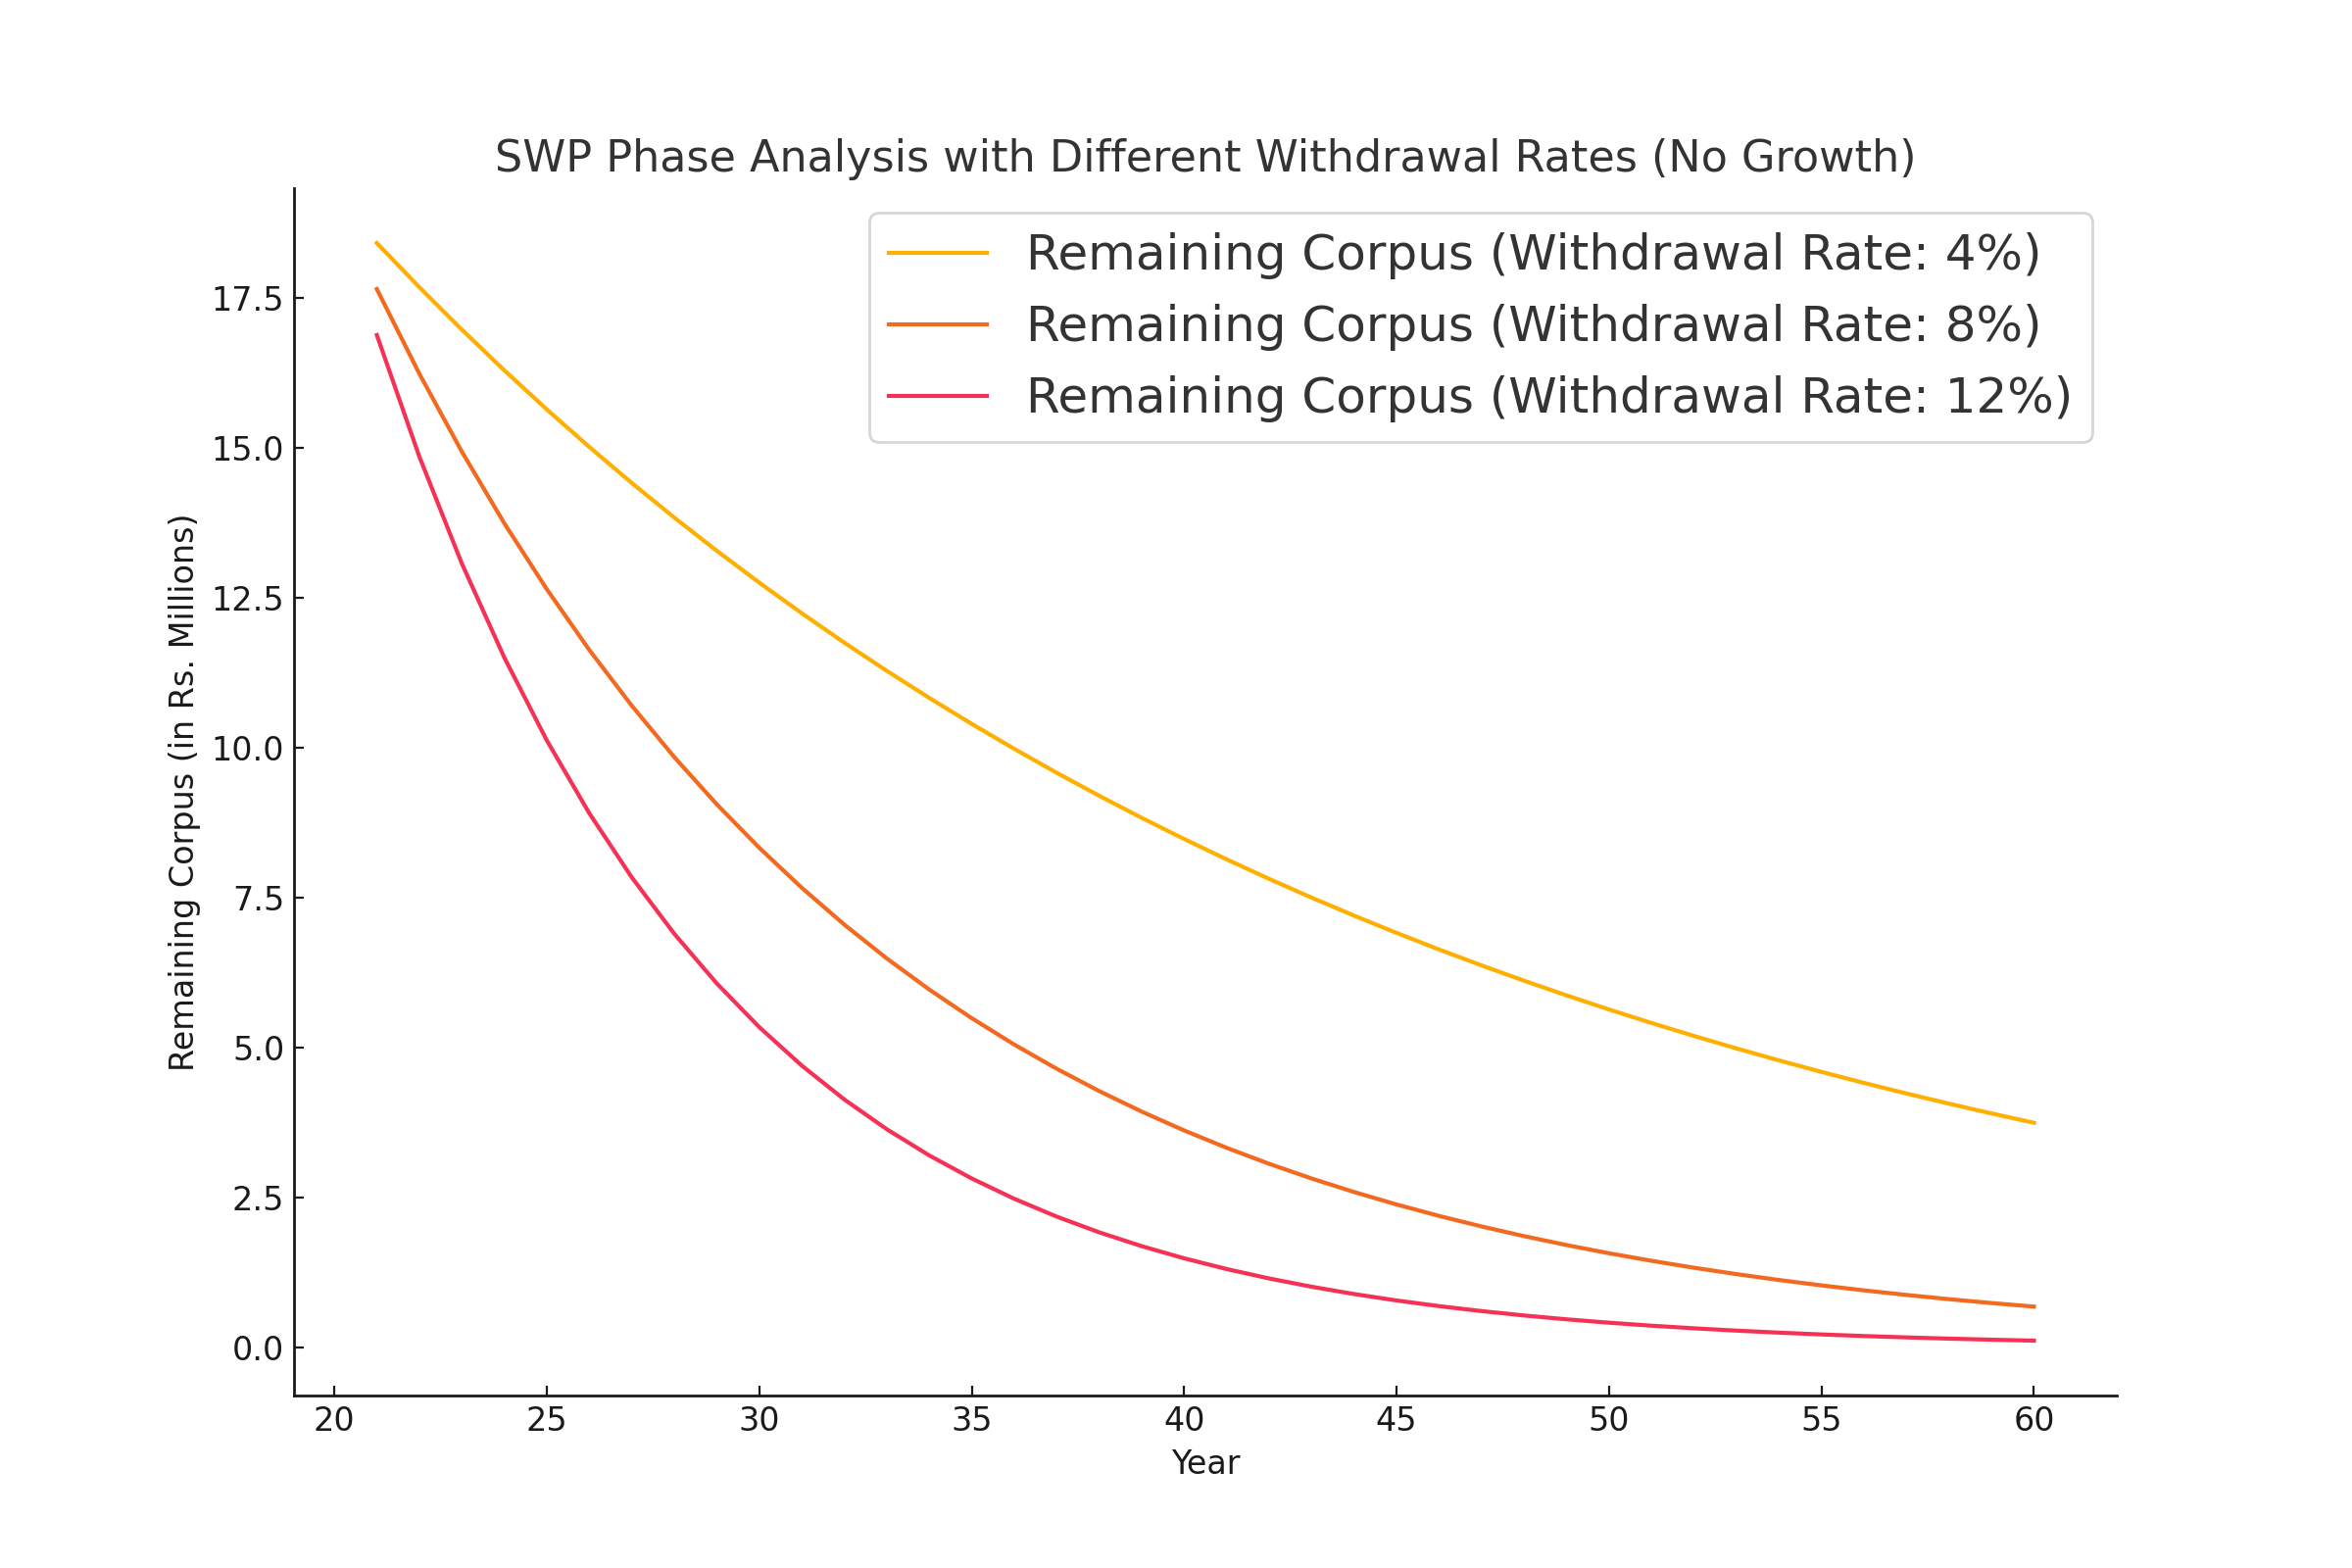
\includegraphics[width=0.6\textwidth]{swp_rate_simulations.png}
	\caption{SWP with Different Withdrawal Rates (No Growth)}
	\label{fig:swp-phase}
\end{figure}

\begin{figure}[!h]
	\centering
	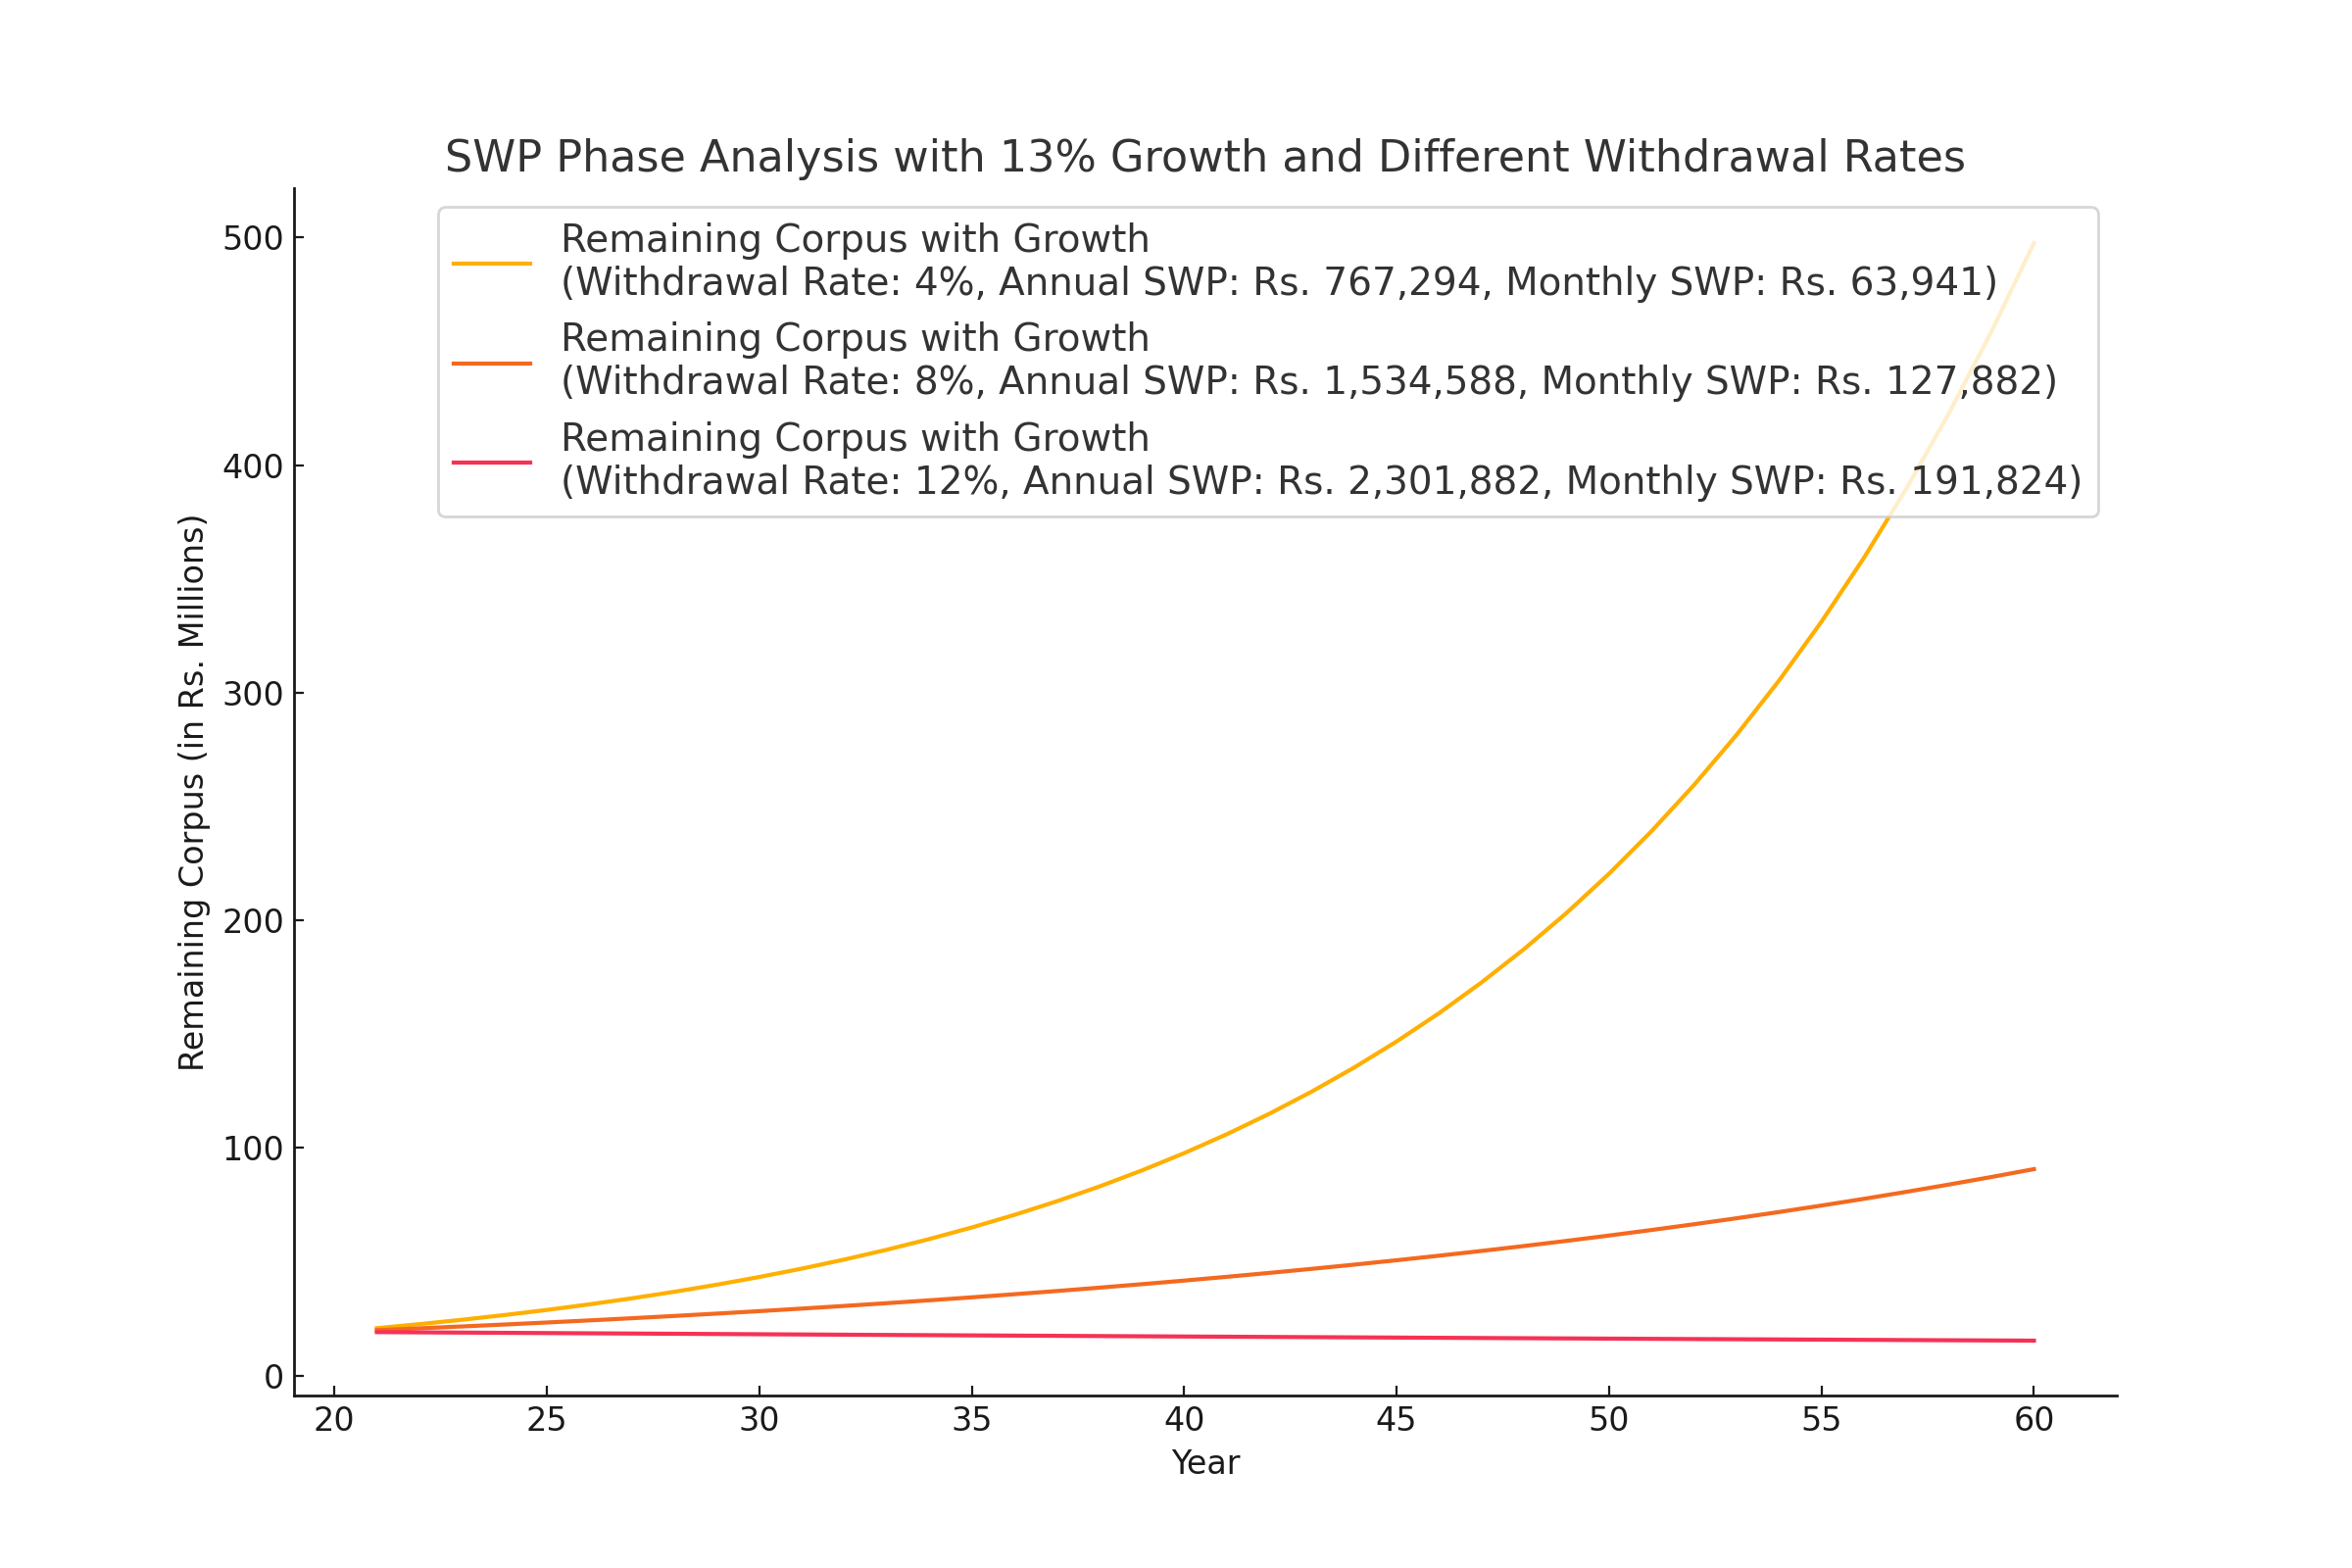
\includegraphics[width=0.6\textwidth]{swp_growth_rate_simulations_with_swp_amounts.png}
	\caption{SWP with 13\% Growth and Different Withdrawal Rates}
	\label{fig:swp-growth-phase}
\end{figure}
		
		The total money saved (Total Investment) grows slowly, but the Accumulated Corpus grows faster because of the interest earned. This phase takes advantage of compound growth, where returns are reinvested, generating higher overall gains. With the 10\% annual انکریمنٹ in savings, the overall corpus grows substantially by the end of the SIP phase. This disciplined approach ensures consistent savings, reducing the impact of market volatility and creating a strong foundation for the next phase.
		
		\section{SWP Phase Analysis}
		In the withdrawal phase (years 21 to 60), money is taken out every year. We tested three rates: 4\%, 8\%, and 12\%. We also included a 13\% growth rate during this phase. Figures~\ref{fig:swp-phase} and~\ref{fig:swp-growth-phase} show what happens to the savings.
	
		
		The SWP phase highlights the sustainability of withdrawals under various scenarios:
		\begin{itemize}
			\item \textbf{4\% Rate}: At this rate, the withdrawal amount is small enough to ensure the corpus lasts throughout the 40 years. The remaining funds continue to grow if the interest exceeds withdrawals.
			\item \textbf{8\% Rate}: This rate increases the withdrawal amount significantly. While this provides higher annual income, it leads to corpus depletion toward the end of 40 years if growth rates are lower.
			\item \textbf{12\% Rate}: At this aggressive rate, the corpus depletes rapidly, often within the first 15 to 20 years, making it unsuitable for long-term planning.
		\end{itemize}
		
		Including a 13\% annual growth rate significantly improves the sustainability of higher withdrawal rates by replenishing the corpus through returns.
		
		\section{Discussion}
		The combined SIP and SWP strategy offers several advantages:
		\begin{itemize}
			\item \textbf{Systematic Discipline}: SIPs enforce a regular savings habit, ensuring consistent contributions irrespective of market conditions.
			\item \textbf{Rupee-Cost Averaging}: Investing a fixed amount during market highs and lows reduces the average cost per unit.
			\item \textbf{Sustainable Withdrawals}: SWPs provide a structured approach to withdrawals, balancing income needs with corpus preservation.
			\item \textbf{Flexibility}: Withdrawal rates can be adjusted based on financial needs and market conditions.
			\item \textbf{Longevity of Savings}: With prudent withdrawal rates, the corpus lasts throughout the withdrawal phase, ensuring financial stability during retirement.
		\end{itemize}
		
		These findings emphasize the importance of maintaining a balance between withdrawal rates and expected growth. Lower withdrawal rates (e.g., 4\%) are ideal for long-term sustainability, while higher rates can provide immediate benefits at the cost of longevity.
		
		\section{Conclusion}
		This report demonstrates the efficacy of combining SIPs and SWPs for achieving long-term financial goals. By adopting a disciplined investment strategy in the SIP phase and following prudent withdrawal rates in the SWP phase, individuals can ensure a stable and sustainable financial future. This approach aligns with the principles of financial planning, emphasizing systematic growth and judicious utilization of resources.
		
		\newpage
		
		% Urdu Report
%		\title{\texturdu{ ایس آئی پی اور ایس ڈبلیو پی رپورٹ}}
%		\author{}
%		\date{\today}
%		\maketitle
%\urdusection{ ایس آئی پی اور ایس ڈبلیو پی رپورٹ}

%\urdutextblock{ایس آئی پی اور ایس ڈبلیو پی طویل مدتی مالی منصوبہ بندی کے لئے دو اہم طریقے ہیں۔ ایس آئی پی کا طریقہ یہ ہے کہ ایک مخصوص رقم کو باقاعدگی سے سرمایہ کاری میں ڈالا جاتا ہے، جس کی وجہ سے ماہانہ یا سالانہ بنیادوں پر سرمایہ بڑھتا رہتا ہے۔ یہ طریقہ اس لئے سودمند ثابت ہوتا ہے کیونکہ کم مقدار میں رقم بھی، وقت کے ساتھ ساتھ، زیادہ منافع کما سکتی ہے۔ اس میں طاقت مجموعی طور پر معمولی مگر مستقل سرمایہ کاری کرنے سے پیدا ہوتی ہے۔ اس دوران، جب سرمایہ کاری کو طویل عرصے تک برقرار رکھا جاتا ہے، تو مختلف اقسام کی منافع کی شرحیں ملنے کے امکانات زیادہ ہوتے ہیں۔ پہلے بیس سالوں میں یہی مسلسل سرمایہ کاری کرنے کا عمل بچت کو مستحکم طور پر بڑھانے میں معاون ثابت ہوتا ہے کیونکہ ہر بار جمع کی گئی رقم پر منافع لگاتار ملتا رہتا ہے۔ اس بڑھتی ہوئی بچت کا اندازہ شکل میں دکھائے گئے گراف سے کیا جا سکتا ہے، جس میں واضح ہوتا ہے کہ وقت گزرنے کے ساتھ سرمایہ لگانے کا اثر کتنی تیزی سے ظاہر ہوتا ہے۔}
%
%\urdutextblock{اس عمل کے دوران کل بچت کی رقم آہستہ آہستہ بڑھتی ہے، لیکن جمع ہونے والے منافع کی وجہ سے اس سرمایہ کی قدر تیزی سے اوپر جاتی ہے۔ یہ اضافہ بنیادی طور پر کمپاؤنڈنگ کے اصول پر مبنی ہے، جس کے تحت وقت گزرنے کے ساتھ منافع خود مزید منافع پیدا کرتا رہتا ہے۔ یہ وہ وجہ ہے کہ جب کوئی شخص لمبے عرصے تک سرمایہ کاری جاری رکھتا ہے تو اس کی مجموعی مالیت روایتی اندازوں سے بڑھ کر بنتی ہے۔ مثال کے طور پر، اگر کوئی فرد ہر مہینے ایک معمولی رقم جمع کرواتا ہے، تو شروعات میں اضافے کی رفتار کم محسوس ہوتی ہے، لیکن کچھ سال گزرتے ہی کل سرمایہ میں تیزی سے اضافہ ہونے لگتا ہے۔}
%
%\urdutextblock{نکالنے کے مرحلے میں ایس ڈبلیو پی کا طریقہ اختیار کیا جاتا ہے۔ اس میں ہر سال کوئی مقررہ یا تناسبی رقم سرمایہ سے نکالی جاتی ہے۔ اس کا مقصد یہ ہوتا ہے کہ فرد کو باقاعدہ طور پر رقم ملتی رہے، جیسا کہ پنشن کے نظام میں ہوتا ہے۔ مختلف نکالنے کی شرحیں اس لئے آزمائی جاتی ہیں کہ اس سے معلوم کیا جا سکے کہ کون سی شرح زیادہ دیر تک سرمایہ کو قائم رکھ سکتی ہے۔ اگر نکالنے کی شرح کم رکھی جائے، جیسے چار فیصد، تو سرمایہ دیر تک محفوظ رہتا ہے اور زیادہ عرصہ تک استعمال ہو سکتا ہے۔ لیکن اگر یہ شرح زیادہ ہو جائے، جیسے بارہ فیصد، تو جمع شدہ سرمایہ چند سالوں میں تیزی سے کم ہونا شروع ہو جاتا ہے۔ جب شرح بہت زیادہ مقرر کی جاتی ہے تو یہ اندیشہ پیدا ہو جاتا ہے کہ سرمایہ مطلوبہ مدت سے پہلے ختم ہو جائے گا، جو کہ ایک غیر مستحکم صورت حال کو ظاہر کرتا ہے۔ مختلف حالات میں تیرہ فیصد کی ترقی کو بھی شامل کیا جاتا ہے تاکہ یہ جانچا جا سکے کہ منافع کی متوقع شرح اور نکالنے کی شرح کا آپس میں کیا تعلق ہے۔ اگر منافع کی شرح نکالنے کی شرح کے قریب ہو یا اس سے زائد ہو تو سرمایہ نسبتاً دیر تک قائم رہ سکتا ہے۔}
%
%\urdutextblock{اسی وجہ سے، ایس آئی پی اور ایس ڈبلیو پی کا امتزاج ایک مؤثر مالی حکمت عملی کے طور پر دیکھا جاتا ہے۔ یہ امتزاج ایک جانب سرمایہ کو منظم انداز میں بڑھانے کے قابل بناتا ہے اور دوسری جانب ایک منصوبہ بند طریقے سے نکالنے کا موقع فراہم کرتا ہے۔ اس طرح، سرمایہ کاری کرنے والا فرد طویل مدت تک اپنے مالی معاملات کو مستحکم رکھ سکتا ہے۔ جمع ہونے والی رقم وقت کے ساتھ بڑھتی ہے، اور جب ضرورت ہو تو مخصوص شرح پر اسے نکالا بھی جا سکتا ہے۔ یہ ایک جامع طریقہ ہے جو نہ صرف مستقبل میں مالی ضروریات کو پورا کرنے میں مدد دیتا ہے بلکہ کسی ہنگامی صورت حال یا ریٹائرمنٹ کے دوران مستقل آمدنی کا ذریعہ بھی بنتا ہے۔ اسی بنا پر رپورٹ میں یہ نتیجہ اخذ کیا گیا ہے کہ ایس آئی پی اور ایس ڈبلیو پی کو یکجا کرنا ایک بہترین حکمت عملی ہے جو مالی استحکام اور طویل مدتی منصوبہ بندی کے اہداف کو بہتر انداز میں حاصل کرنے میں معاون ثابت ہوتی ہے۔}

%\urdutextblock{ایس آئی پی اور ایس ڈبلیو پی طویل مدتی مالی منصوبہ بندی کے دو اہم طریقے ہیں۔ ایس آئی پی میں باقاعدگی سے سرمایہ کاری کی جاتی ہے، جس سے وقت کے ساتھ بچت میں اضافہ ہوتا ہے۔ کمپاؤنڈنگ کی بدولت جمع ہونے والا منافع خود مزید منافع پیدا کرتا ہے، جس سے سرمایہ تیزی سے بڑھتا ہے۔}
%
%\urdutextblock{ایس ڈبلیو پی نکالنے کے مرحلے میں استعمال ہوتا ہے، جہاں ہر سال طے شدہ رقم نکالی جاتی ہے۔ کم شرح نکالنے سے سرمایہ طویل عرصے تک محفوظ رہتا ہے، جبکہ زیادہ شرح جلدی سرمایہ ختم کر سکتی ہے۔ تیرہ فیصد کی ترقی کی شرح سرمایہ کو زیادہ دیر تک برقرار رکھنے میں مددگار ثابت ہو سکتی ہے، بشرطیکہ یہ نکالنے کی شرح سے زیادہ ہو۔}
%
%
%
%\urdutextblock{ایک سادہ مثال یوں ہے کہ ایک باپ اپنے بیٹے کے لئے بیس سال تک ہر سال ایک مخصوص رقم سرمایہ کاری میں ڈالتا ہے۔ پہلے سال وہ ایک لاکھ بیس ہزار روپے لگاتا ہے، اگلے سال اس رقم میں دس فیصد کا معمولی اضافہ کیا جاتا ہے، اور یوں یہ رقم آہستہ آہستہ بڑھتی رہتی ہے۔ ان بیس سالوں میں کل چھ لاکھ ستّر ہزار روپے کے قریب رقم جمع کروائی جاتی ہے، لیکن منافع اور کمپاؤنڈنگ کی وجہ سے یہ کل سرمایہ تقریباً انیس لاکھ روپے سے اوپر پہنچ جاتا ہے۔ اس عرصے میں اصل فائدہ کمپاؤنڈنگ کا ہوتا ہے، جس میں ہر سال کا منافع اگلے سال مزید منافع پیدا کرتا ہے۔}
%
%\urdutextblock{بیس سال کے بعد جب بیٹا اپنی جوانی میں قدم رکھتا ہے تو وہ اسی جمع شدہ سرمائے سے باقاعدہ رقم نکالنا شروع کرتا ہے۔ اس مرحلے میں ایس ڈبلیو پی کا طریقہ اپنایا جاتا ہے، جس کے تحت ہر سال طے شدہ یا خاص تناسب سے پیسے نکالے جاتے ہیں۔ مثال کے طور پر، اگر کوئی چار فیصد کی شرح نکالنے کا فیصلہ کیا جائے تو ہر سال کی رقم زیادہ تو نہیں ہوتی، لیکن سرمایہ دیر تک چلتا رہتا ہے، کیونکہ نکالی جانے والی رقم نسبتاً کم ہوتی ہے اور باقی سرمایہ اپنی رفتار سے بڑھتا رہتا ہے۔ اگر آٹھ فیصد سالانہ نکالا جائے تو جیب خرچ تو بڑھ جاتا ہے، لیکن ہو سکتا ہے کہ چالیس سال کی مدت کے آخری حصے تک سرمایہ اتنا زیادہ نہ بچے۔ بارہ فیصد کی شرح زیادہ تیز رفتار سے سرمایہ کم کرتی ہے، اور عموماً پندرہ سے بیس سال کے اندر ہی بڑی حد تک ختم ہونے کا خدشہ رہتا ہے۔ البتہ اگر سرمایہ کاری پر تیرہ فیصد کا سالانہ منافع بھی مل رہا ہو تو نسبتاً زیادہ نکالنے کی شرحیں بھی کچھ دیر تک سنبھالی جا سکتی ہیں، کیونکہ نئے منافع سے سرمایہ کی کمی پوری ہونے کے امکانات بڑھ جاتے ہیں۔}
%
%\urdutextblock{اس ساری مثال سے معلوم ہوتا ہے کہ ایس آئی پی اور ایس ڈبلیو پی کو ملا کر استعمال کرنا ایک مضبوط مالی حکمت عملی بن جاتا ہے۔ ایس آئی پی میں باقاعدگی سے رقم ڈالی جاتی ہے، جس سے سرمایہ تشکیل پاتا رہتا ہے، جبکہ ایس ڈبلیو پی مرحلے میں اتنی رقم نکالی جاتی ہے جو جیب خرچ یا دیگر ضروریات پوری کرنے کے لئے کافی ہو۔ اگر نکالنے کی شرح احتیاط سے رکھی جائے تو سرمایہ زیادہ عرصے تک قائم رہتا ہے اور بیٹے کو مستقبل میں بھی استعمال کے لئے مناسب رقم دستیاب ہوتی رہتی ہے۔ یہ طریقہ کار منظم سیونگ اور منصوبہ بند نکالنے، دونوں پہلوؤں کو یکجا کر دیتا ہے، جس کی بدولت لمبے عرصے تک مالی تحفظ اور نسبتاً خودمختاری برقرار رکھی جا سکتی ہے۔}

\urdutextblock{ذیل میں ایک مفروضے کی بنیاد پر وہی طویل مدتی سرمایہ کاری کی حکمتِ عملی بیان کی گئی ہے، جس میں باپ بیٹے کے مابین مالی ذمہ داری کا مستقل نظام تشکیل پاتا ہے۔ البتہ یہاں ہم نے دو اضافی نکات کا اندراج کیا ہے: ایک تو یہ کہ سرمایہ کاری کے اس منصوبے میں ہر سال ماہانہ جمع ہونے والی رقم میں ۰۱ فیصد کا اضافہ (انکریمنٹ) ہوتا ہے اور دوسرا یہ کہ ۰۲ سال کے بعد حاصل ہونے والے کل سرمائے سے سالانہ ۴ فیصد نکالا جاتا ہے ۔ نیز سالانہ منافع کی اوسط شرح کو ۳۱ فیصد تصور کیا گیا ہے۔ ان اعدادی مفروضات کی روشنی میں ہمارا ہدف یہ ہے کہ بیٹے کے جوان ہونے پر اس کے پاس نہ صرف ایک معقول سرمایہ موجود ہو، بلکہ اس سے باقاعدہ رقوم نکالنے کا ایسا لچک دار نظام بھی ہو جو روزمرہ اخراجات اور ضروریات کو پورا کرنے کے ساتھ ساتھ بنیادی سرمائے کو مسلسل بڑھاتا رہے۔}

\urdusection{ابتدائی بیس سال: باقاعدہ سرمایہ کاری اور کمپاؤنڈنگ کا امتزاج}

\urdutextblock{ماہانہ جمع ہونے والی رقم اور سالانہ اضافہ  
	شروع میں باپ ہر مہینے دس ہزار روپے کی رقم جمع کرتا ہے۔ اگلے سال اس رقم میں ۰۱ فیصد کا اضافہ ہوتا ہے، یعنی دوسرے سال میں یہ ماہانہ رقم تقریباً گیارہ ہزار روپے ہو جاتی ہے۔ اس سے اگلے سال مزید ۰۱ فیصد کے اضافے سے یہ رقم تقریباً بارہ ہزار ایک سو روپے تک پہنچ جاتی ہے، اور یہ سلسلہ یوں ہی بڑھتا جاتا ہے۔ اس طرح پہلے سال کے اختتام تک مجموعی طور پر تقریباً ایک لاکھ بیس ہزار روپے جمع ہوتے ہیں، جب کہ دوسرے سال کی سالانہ رقم میں واضح اضافہ نظر آتا ہے۔ تیسرے، چوتھے اور پانچویں سال میں بھی اسی اضافے کے ساتھ سرمایہ کاری جاری رہتی ہے، جس کے نتیجے میں مجموعی سرمایہ ہدف کی جانب تیزی سے بڑھتا رہتا ہے۔}

\urdutextblock{۳۱ فیصد سالانہ اوسط منافع 
	اس پورے عرصے میں ہم نے یہ فرض کیا ہے کہ سرمایہ کاری پر اوسط سالانہ منافع ۱۳ فیصد کے قریب رہتا ہے۔ یہ منافع ہر سال کے آخر میں بنیادی رقم میں ضم ہو کر اگلے سال کی سرمایہ کاری کے ساتھ مل کر کمپاؤنڈنگ کو تقویت دیتا ہے۔ چنانچہ جوں جوں سرمایہ بڑھتا جاتا ہے، اس پر ملنے والا منافع بھی نسبتاً زیادہ ہو جاتا ہے، جس سے مجموعی پورٹ فولیو تیزی سے آگے نکلتا ہے۔}

\urdutextblock{بیس سال کی تکمیل پر مجموعی سرمایہ  
	اس حکمتِ عملی کے تحت، جب بیس سال مکمل ہونے کو آتے ہیں، تو باپ نے ہر سال ماہانہ بنیادوں پر رقم جمع کی ہوتی ہے، جس میں ہر سال ۰۱ فیصد انکریمنٹ آتا رہتا ہے۔ ۳۱ فیصد سالانہ منافع کے ساتھ یہ پورٹ فولیو ترقی کرتا ہوا کئی گنا بڑھ جاتا ہے۔ مثال کے طور پر کسی ایک سال میں باپ نے سالانہ ڈیڑھ لاکھ روپے کے قریب رقم جمع کروائی تو اس پر ملنے والا منافع بھی اسی تناسب سے پورٹ فولیو کو تقویت بخشتا رہا۔ بیسویں سال تک آتے آتے یہ مجموعی سرمایہ عام اندازوں کے مطابق پندرہ سے بیس لاکھ روپے یا اس سے بھی زائد تک پہنچ سکتا ہے، جیسا کہ بیسویں سال میں یہ سالانہ جمع ہونے والی رقم سات لاکھ تینتیس ہزار نو سو روپے تک پہنچ جاتی ہے اور کل جمع شدہ رقم ۱ کروڑ اکوانوے لاکھ بیاسی ہزار تین سو ایکاون روپے بن چکی ہے۔ }

\urdusection{اکیسویں سال سے آگے: ۴ فیصد سالانہ نکالنے کا نظام}

\urdutextblock{ 
	جب بیٹا بیسویں عشرے میں داخل ہوتا ہے تو والد اس پورٹ فولیو سے رقوم نکالنے کا ایک نیا سلسلہ شروع کرنے کے قابل ہو جاتا ہے۔ اس میں ہر سال صرف ۴ فیصد کے قریب رقم نکالی جاتی ہے، تاکہ بنیادی سرمایہ محفوظ رہے اور اگلے سالوں میں مزید ترقی کرتا رہے۔  
	مثال کے طور پر اگر بیسویں سال کے اختتام پر پورٹ فولیو کی مالیت فرض کریں ۱ کروڑ روپے تھی تو اکیسویں سال میں ۴ فیصد کے حساب سے تقریباً  ۴ لاکھ روپے سالانہ نکالے جا سکتے ہیں۔ جوں جوں سرمایہ اور منافع بڑھتا جاتا ہے، یہ رقم بھی ہر سال بڑھے گی اور اس سے روزمرہ اخراجات کو آسانی سے پورا کیا جا سکتا ہے۔}

\urdutextblock{بائیسویں سے تیسویں سال تک اخراجات میں تدریجی اضافہ  
 کے تحت ہر سال ۴ فیصد نکالنا ہوتا ہے، جب کہ باقی رقم پورٹ فولیو میں دوبارہ لگ کر ۳۱ فیصد کے قریبی منافع سے مزید بڑھتی رہتی ہے۔ یوں اگر بائیسویں سال نکالی جانے والی رقم سات لاکھ روپے تک پہنچ جاتی ہے تو اس کی وجہ یہ ہے کہ پورٹ فولیو بڑھ کر کہیں ۲ کروڑ روپے کی رینج میں آ جاتا ہے۔ اس طرح بیٹے کو ہر سال اخراجات پوری کرنے کے لئے مناسب رقم ملتی رہتی ہے، اور اصل سرمایہ بھی تیزی سے گھٹنے کے بجائے مسلسل تقویت پاتا رہتا ہے۔}

\urdutextblock{
	جب یہ سلسلہ تیس چالیس سال آگے چلتا جاتا ہے تو سالانہ نکالی جانے والی رقم بھی دس لاکھ سے پندرہ لاکھ روپے، بلکہ اس سے بھی اوپر پہنچ سکتی ہے، اگر سالانہ منافع (۳۱ فیصد) برقرار رہتا ہے اور صرف ۴ فیصد نکالا جاتا ہے تو پورٹ فولیو ہر گزرتے سال بڑھتا چلا جاتا ہے۔ اس کا فائدہ یہ ہوتا ہے کہ پچاسویں اور ساٹھویں سال تک جاتے جاتے بھی اخراجات کی خاطر ایک معقول رقم نکالی جا سکتی ہے، جبکہ اصل سرمایہ مزید بڑا ہو جاتا ہے۔ چاسویں سال میں یہ رقم تئیس لاکھ روپے سالانہ تک پہنچ سکتی ہے اور پھر ساٹھویں سال کے قریب پینتیس لاکھ روپے سالانہ اخراج کا ہدف بھی ممکن ہو جاتا ہے، جب کہ مجموعی سرمایہ کئی گنا آگے نکل چکا ہوتا ہے۔}

\urdusection{نتیجہ}

\urdutextblock{		ہر مہینے ایک مخصوص رقم جمع کرنے کی عادت کو برقرار رکھیں، اور اگر ممکن ہو تو ہر سال اس میں ۰۱ فیصد کا اضافہ کر دیں۔ اس طریقے سے آپ اپنے پورٹ فولیو کو افراطِ زر اور دیگر مالیاتی دباؤ سے محفوظ رکھنے میں ایک حد تک کامیاب ہوتے ہیں۔  
	طویل مدتی نظر اور کمپاؤنڈنگ کا فائدہ  
	لمبے عرصے تک سرمایہ کاری کرنے سے کمپاؤنڈنگ کا عمل طاقت پکڑتا ہے۔ ۳۱ فیصد جیسا منافع اگر مسلسل ملتا رہے تو ۰۲ سال بعد ہی آپ کے پاس معقول سرمایہ جمع ہو سکتا ہے۔  

	ایک بار جب معقول رقم جمع ہو جائے تو ہر سال ۴ فیصد جیسا نسبتاً کم تناسب نکالنے کی حکمتِ عملی اپنانے سے بنیادی سرمایہ کو زیادہ تیزی سے گھٹنے سے محفوظ رکھا جا سکتا ہے۔ یوں اضافی منافع سال بہ سال سرمائے کو بڑھاتا جاتا ہے۔  
	خاندانی مالی ذمہ داری کی مضبوطی  
	ایک ایسا باقاعدہ نظام ترتیب پاتا ہے جس میں باپ کی جانب سے کی گئی طویل عرصے کی کوششیں ضائع نہیں جاتیں۔ بیٹا جوان ہو کر باآسانی اپنے اخراجات پورے کرنے کے ساتھ ساتھ اپنے خوابوں کی تکمیل کے لئے مناسب سرمائے سے مستفید ہو سکتا ہے، جب کہ بنیادی سرمایہ مستقل طور پر بڑھتا رہتا ہے۔}

\urdutextblock{یہی طریقۂ کار خاندانوں کو طویل المیعاد بنیادوں پر ایک مستحکم اور محفوظ مالی مستقبل فراہم کرنے میں معاون ثابت ہوتا ہے۔ ماہانہ سرمایہ کاری اور اس میں بتدریج سالانہ اضافہ، ۳۱ فیصد کے اوسط منافع اور پھر ۴ فیصد کے سالانہ اخراج کے امتزاج سے، ایک ایسی توازن یافتہ صورتِ حال قائم کی جا سکتی ہے جو روزمرہ ضروریات کے ساتھ ساتھ آنے والی نسلوں کے لئے بھی مالی تحفظ فراہم کر دیتی ہے۔}

	\end{document}
	